\chapter{Methodology}
\label{ch:method}

% \begin{figure}[htb!]  % Changed from figure* to figure unless you specifically need double-column
%     \centering
%     % \begin{subfigure}[b]{1.5\textwidth} 
% 	\centering
% 	\resizebox{1.5\textwidth}{!}{
% 		
\begin{tikzpicture}[
    node distance=8mm and 0mm,
    block/.style={draw, fill=blue!10, rounded corners, minimum width=3cm, minimum height=1cm, align=center},
    arrow/.style={-Stealth, thick},
    shapenode/.style={ellipse, draw, fill=red!10, minimum width=2cm},
    legendbox/.style={draw, fill=white, font=\small}
]

% Input
\node (input) {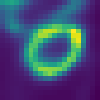
\includegraphics[width=1.2cm]{sagittal_input.png}};
\node[above=1mm of input, font=\footnotesize] {Input SPECT Volume};

% Preprocessing
\node[block, below=of input] (preprocess) {Preprocessing \\ (Normalization, Denoising)};
\draw[arrow] (input) -- (preprocess);

% Shape Prior Path
\node[shapenode, left=of preprocess, xshift=-1cm] (shape) {Statistical Shape Model};
% \draw[arrow] (shape) -- (priors);
% \draw[arrow, dashed] (input.west) -- ++(-6cm,0) |-  (shape.north);
% \draw[arrow, dashed] (input.west) -- ++(-6cm,0) coordinate (temp) -- (temp|-shape.north) -- (shape.north);
\coordinate (temp) at ($(input.west) + (-6.05cm, 0)$);
\coordinate (drop) at ($(shape.north) + (-0cm, 0.1)$);

\draw[arrow, dashed] (input.west) -- (temp) -- (drop) -- (shape.north);


% Transformer Encoder
\node[block, below=of preprocess] (encoder) {nnFormer Encoder};
\draw[arrow] (preprocess) -- (encoder);
% \draw[arrow, dashed] (shape.east) -- (preprocess.west);

% Fusion
\node[block, below=of encoder] (fusion) {Feature Fusion \\ (nnFormer Features \ensuremath{\oplus} Shape Priors)};\draw[arrow] (encoder) -- (fusion);
\draw[arrow] (shape.south) |- ([xshift=-5mm]fusion.west) -- (fusion.west);

% Decoder
\node[block, below=of fusion] (decoder) {nnFormer Decoder};
\draw[arrow] (fusion) -- (decoder);
\draw[arrow, dashed] (encoder.east) -| ++(2cm,0) |- (decoder.east);

% Output
\node[below=of decoder] (output) {
\includegraphics[width=1.2cm]{sagittal_gt.png}};
\node[below=1mm of output, font=\footnotesize] {LV Segmentation Mask};
\draw[arrow] (decoder) -- (output);


% Ensure all content is within bounds
\useasboundingbox (current bounding box.south west) rectangle ([xshift=6cm]current bounding box.north east);

\end{tikzpicture}
% 	}
% 	\caption{\centering Network architecture pipeline}
% 	\label{fig:network_pipeline}
% \end{figure}

\section{Overview}
The main goal of the research is to propose a comprehensive and strong method which is desiggned specifically to significantly improve the accuracy of the segmentation of MPI using SPECT for the Left ventricle. The precise segmentation of MPI SPECT images is extremely critical for the detection and the assessment of CAD. However, the task of achieving a high accuracy in segmentation poses a number of challenges due to a multitude of inherent limitations of MPI SPECT data, such as low signal-to-noise ratio (SNR) partial volume affects, substantial noise because of the poisson statistics, motion artifacts and, obviously, the anatomical variability among different patints. 

In order to address these challlenges, the proposed research amalgamates advanced approaches in the field of deep learning, more specifically utilizing the transformer based architecture known as nnFormer \cite{10.1109/TIP.2023.3293771}, which is combined with an innovative idea of using statistical shape prios. The nnFormer architecture is chosen because of the ability of it of capturing both the ocal and the global information or contextual relationships in volumetric data as opposed to traditional CNNs which only capture local information. nnFormer leverages the local volume-based (LV-MSA) and the global volume-based (GV-MSA) multi-head self-attention mechanisms very efficiently in a unified method. These modules of the transformer architecture very effectively encode the longg-range dependencies which are extremely important for better segmentation accuracy specifically in medical imaging where they are characterized by indistinct boundaries.

Simultanously, the SSP are merged into the segmentation pipeline in order to improve the anatomical consistency of the model. SSPs provide the DL model with a mathematical model which captures the probabilistic variability off the LV that are derived from the data annotated by experts. This SSP methos employes an advanced technique of optimization such as Mahalanobis distance based regularization and the Kullback-Liebler (KL) divergence in order to refine the segmentation boundaries. This way the outputs of the segmentation model maintain plausibile anatomical outputs, which improves the segmentation accuracy even when the input data is incomplete or ambiguous. The combination of nnFormer and SSP provides us with a novel hybrid architecture. 

This hybrid approach leverages not only the strengths of DL models in extracting complex and heirarchical feature representations from volumetric data, but also the advantages of SSPs in mantaining consistent anatomies. This approach also adressess the limitations of the existing methods, which include inefficient generalization capability and dependencies of large, precisely annotated data for training. It also mitigates the impact of a number of different imaging artifacts and the noise, which enhances the overall relaibility on the segmentations.

Extensive procedures for training involving efficient optimization strategies such as Adam, and specifically segmentation tailored loss such as the DiceCE loss, are implemented in order to ensure stable performance across a diverse set of paatients. The training and the validation aspects are conducted rigorously using an extensive dataset of MPI SPECT which consists of diverse collimation methods and demograhics of the patients which improves the generalization capability of the method. Extensive setups of computation which leverage high performance GPU computing environments ensure efficient training and inference of the model. Comprehensive evalaution metrics are utilized in order to quantitatively validate the performance of the segmentation. These metrics include precision, recall, intersection over union (IoU) and Dice coefficient. These metrics provide an extremely in-depth insights into the capability of the method to handle real-world variability and complex scenarios.

In a summary, the proposed methodology contibutes to not only a significant advancement in the division of cardiac image segmentation but also provides a practical and robust solution which is applicable in a clinical environment. The combination of nnFormer and SSP ensures reliable and precise segmentation having clinically meaningful results, which paves the way for better and improved diagnosis and patient outcoms in CAD management.


\section{Data Acquisition and Preprocessing}

The MPI dataset which is utilized in this research was acquired using SPECT. This acquired dataset consists of volumes from a total of 74 patients, which are carefully selected in order to represent the diverse demographic and the characteristics of the clinic. The popultion of the patients inclued individuals with varying age groups, physiological conditions and gender distributions in order to ensure the relaibility, robustness and generalizability of the model. Multiple different radiotracers were employed in the process of acquiring the MPI SPECT, specifically agents labled by technetium-99m(Tc) such as Tc Tetrofosmin and TC Sestamibi, and also the thallium 201 chloride (T1 Chloride). 

Each of these radiotraces offer unique properties in imaging thereby providing a comprehensive coverage of all the possible clinical scenarios which are encountered in everyday diagnostice. The dataset was recorded using multiple different collimation methods and also different imaging configurations, including muti-pinhole (MPH), low-energy high-resolution (LEHR), CardioC, CardioD collimators. These various imaging techniues simulate the real-world variability in the clinical practices and pose very distinct challenges for segmentation models because of the variations in spatial resolution, noise characteristics and the sensitivity. Specifically, the dataset consists of 40 patients who are imaged with mixed black-box collimators, 8 patients each images using MPH, CardioC and CardioD, and 10 patients images using LEHR collimators. This comprehensive approach ensures that the data consists of a wide rane of both the quality of the image and also the imaging artifacts which are typically observed in a clincal setting.

Each of the patient went through very rigorous imaging procedures which are adhering strictly to standard protocals of acquisition in clinics. The patients were administered the mentioned radiopharmaceuticals intravenously which was followed by image acquisition after the standardized waiting period that allows sufficient tracer uptake in the myocardial tissue. The image acquisition protocols were varying based on the collimation method which was emploed. For example imaging with the MPH collimator a very specific step-and-shoot helical trajectories, on the other hand the stationary collimator positions were employed for the other collimators which creates different spatial sampling patterns and different challenges to image reconstruction. AFter the acquisition of the raw data, a number of precprocessing techniques were employed in ordder to prepare the data for the subsequent segmentation analysis. The preprocessing pipeline was developed in order to address a number of inherent issues with the imaging and to optimize the data quality for better segmentation outcomes.

The preprocessing steps began with the correction of the attenuation utilizing the TeraTomo reconstruction algorithm \cite{Nagy2013}, which majorly removed the attenuation artifacts which are caused by the soft bone and tissue structures. This step is very essential in order to ensure the uniformity in the ditribution representation of the tracer across the myocardial tissue, hence improving the segmentation accuracy. In some cases where the attenuation correction data was not available, an Ordered Subset Expectation Maximization (OSEM) algorithm \cite{Hudson1994} was used in order to reconstruct the full field-of-view (FOV) volumes, providing us with data with robust handling of poisson noise and preserving essential details of the image. 

In order to improve the image quality even more, noise reduction techniques are employed, specifically targeting the reduction of the poisson noise which is the most prominent in MPI SPECT imaging due to the low cound of the photons. More advanced filtering methods were also employed such as the Gaussian smoothing and the adaptive median filtering in order to balance the noise reduction with the preservation of important boundaries anatomically and the structural details. The partial volume effects (PVE), which majorly has an impact on the accuracy of the segmentation because of blurring tissue boundaries, were adressed systematically using dedicated PV correction tecnhiques and deconvolution techniques. These methods restored the sharpness in the images and enhanced the delineation of th myocardial boundaries, especially in the regions which have complex anatomical structures.

The images that are the result of the above preprocessing are made to go through further normalization procedures in order to ensure consistency in the scales of intensity across all the datasets which helps in haveing more robust training of the final segmentation models. Standardization of the intensities of the voxels involved scaling the pixel intensity distribution in order to have a mean of zero and a unit variance, which significantly improves the numerical stability, which in-turn helps the convergence of the DL models.

All the data preprocessing steps are performed in a very structured and repeatable framewor, usin scripts that are custom developed in Python and specilized libraries for medical imaging and DL such as PyTorch, TorchIO and Scikit-learn. The comprehensive documentation of the preprocessing parameters and the configurations was nicely maintained so as to ensure the transparancy and the reproducibilit of the methodology. The final dataset after the preprocessing provided us with a very high-quality and standardized input data for the training, validation and the testing of the DL models. The careful handling of the whole data acquisition pipeline ensuring the variability and the rigorous preprocessing ensured optimal MPI SPECT image preparation which maorly enhanced the accuraacy and the relaiability of the segmentation which was obtained from the hybrid model.


\section{Detailed Description of nnFormer Architecture}

The nnFormer architecture introduces an innovative advancements in the field of medical image segmentation, which is specifically designed in order to address the limiations that are faces by the traditional CNNs. nnFormer does it by efficiently capturing both the local and the global spatial relationships in the volumetric medical data. This section gives a very detailed description of the architecture explaining the components, their integration, and the rationale behind the usage of the components in the spicified manner.

\subsection{Overall Architecture}

The nnFormer architecture follows a structure that is very much used in the image segmentation field. It follows a U-shaped encoder decoder architecture which is inspired by the widely used U-Net. This choise of the structure helps in efficient learning of the detailed local features, all the while preserving and leveraging the global contexutual information across multiple scales of resolution. The nnFormer architecture comprises of three main components: an encoder, a bottleneck and a decoder which are all interconnected via skip connections.

\subsection{Encoder}
The encoder of nnFormer starts with an embedding layer, which consists of multiple convolutional layers with very small kernel sizes, typically using 3x3x3. This is followed by Gaussan Error Linear Units (GELU) activation and then ends with a normalization layer. This initial convolutional based embedding transforms the input volume into a higher dimentional featurespace which encodes the low-level spatial detailed, which are necessary for subsequent processing, very efficiently. After the embedding layer, the encoder uses a Local Volume-based Multi-hea Self-attention (LV-MSA) blocks. These LV-MSA blocks are designed so that they can capture the local spatial dependencies within the segmented volumes, which significantly reduces the computaitonal compllexity of the model as compared to the conventional global self-attention mechanisms. 

Each of the LV-MSA blocks is further comprised of successive layers of transformer modules in order to use attention mechanisms to effectively model the ver intricate local intractions contexxually. The encoder also combines very strategically placed downsampling convolutional layers which reduces the spatial dimensions of the feature maps while at the same time progressively increasing the depth of the feature map. This downsampling process helps the extraction of the heirarchical features in a more abstract way and on a global scale based representations at lower resolutions, which are essential for capturing the borader variations and anatomical structures.

\subsection{Bottleneck}
In the center of the nnFormer there is a bottleneck. This bottleneck has global volume-based multi-head self-attention (GV-MSA) mechanisms. Contrary to the LV-MSA, the GV-MSA provides with a significantly bigger receptive field which captures the long-range dependencies across the whole global context of the volumetric feature map. This increased area of the receptive field is essential at this stage in order to allow the network to achieve a comprehensive understanding of the global representation and the anatomical structures, improving the overall segmentation accuracy. The bottleneck very effectively combines the compllex spatial dependencies and also the high level features which are exracted by the encoder. Thi serves as a robust foundation for the decoder for accurate and consistent output during the decoding.

\subsection{Decoder}
The decoder is, in a way, mirrored version of the encoder it also employs LV-MSA blocks but coupled with convolutional upsampling, instead of the downsampling, or so-called transposed convolution. This restores the spatial resolution of the feature maps gradually to the original dimenstions of the input. Each step of the upsampling process in the decoder is designed so as to reconstruct the detailed anatomical information by combining the high resolution detail captured sptially from the corresponding encoding stages via skip connections. 

A prime innovation of the nnFormer is the use of the skip attention mechanisms, in place of he traditional concatenation or summation which is typically used in skip connection mechanisms. These skip connections very selectively integrates the features of the encoder with the corresponding features of the decoder, which are guided by the attention weights that highlight relevant spatial features dynamically and hence suppress the irrelevant features. This selective combinaton majorly improves the precision of the segmentation, specifically in the areas where the clear anatomical delineation is very challenging due to the noise and artifacts.

\subsection{Attention Mechanisms}
nnFormerutilizes two different types of attention mechanisms: the Local Volume-based Multi-head Self-attention (LV-MSA) and Global Volume-based Multi-head Self-attention (GV-MSA). LV-MSA very effficiently models the local spatial dependencies by partitioning the feature maps into manageable patches of volumes, which reduces the computational complexity without sacrificing a lot of the performance of the attention mechanism. In contrast to this, GV-MSA models the global interactions spatially across the entire volumetric feature maps, which are essential for capturing the large scale anatomical structural integrity and the contextual relationships. Both of thse attention mechanisms use multi-head configurations which enable parallel computations of attention across multiple representational subspaces. This multi-ha design greatly improves the capability of the network in order to concurrently capture very diverse spatiall relationships and the interactions at multiple scales hence thereby improving the segmentation accuracy.

\subsection{Integration and Optimization}
The amalgamation of LV-MSA, GV-MSA and the convolutional operations in the nnFormer is very carefully optimized in order to leverage the strength of each of these methods. The convolutional layers provide the efficient encoding of the low level spatual features, while the LV-MSA and the GV-MSA collectively capture both the complex spatial contexts and the long-range dependencies which are crucial for the precise and robust segmentaiton. Optimization of the nnFormer involves a specialized loss function called the Dice cross entropy loss (DiceCELoss). This loss function objectivises a high segmentation accuracy while maintaining a reliable realisic plausibility, which effectively guides the learning process towards more generalizable models acrosss diverse imaging conditions.


In conclusion, the nnFormer architecture represents a very sophisticated segmentation framework which is specifically tailored for medical imaging systems. The innovative design of the architecture and the advaned methods of attention overcomes the traditional limiations of segmentation models by effectively using optimization techniques across components ensuring accurate, robust and clinically meaningfull segmentation outputs.